\documentclass[12pt]{article}
\usepackage[utf8]{inputenc}
\usepackage[spanish]{babel}
\usepackage[none]{hyphenat} % no cortar las palabras
\usepackage[margin=25mm]{geometry}
    \hyphenation{thatshouldnot}
\usepackage{graphicx}
    \graphicspath{{images/}}
\usepackage{tikz}
    \usetikzlibrary{shapes,arrows,positioning}
\usepackage{float}
\usepackage{listings} % for codeblocks
\renewcommand{\lstlistingname}{Código}% Listing -> Algorithm
\usepackage{parskip}
\usepackage{hyperref}

\definecolor{codegreen}{rgb}{0,0.6,0}
\definecolor{codegray}{rgb}{0.5,0.5,0.5}
\definecolor{codepurple}{rgb}{0.58,0,0.82}
\definecolor{backcolour}{rgb}{0.95,0.95,0.92}

\lstdefinestyle{mystyle}{
    backgroundcolor=\color{backcolour}, commentstyle=\color{codegreen},
    keywordstyle=\color{magenta},
    numberstyle=\tiny\color{codegray},
    stringstyle=\color{codepurple},
    basicstyle=\ttfamily\footnotesize,
    breakatwhitespace=false,
    breaklines=true,
    captionpos=b,
    keepspaces=true,
    numbers=left,
    numbersep=5pt,                  
    showspaces=false,                
    showstringspaces=false,
    showtabs=false,                  
    tabsize=2,
    frame = single, 
}
\lstset{style=mystyle}

\begin{document}

\begin{titlepage}
    \centering
    {\scshape\LARGE Universidad Católica de Santa María \par}
    \vspace{3em}
    \includegraphics[width=0.25\textwidth]{$HOME/.config/latex/images/Escudo-UCSM.png}\par\vspace{3em}
    \vspace{1cm}
    {\scshape\Large Escuela Profesional de Ingeniería Electrónica \par}
    \vspace{1.5cm}
    {\huge\bfseries Informe 4NEC2\par}   % título del proyecto
    \vspace{2cm}
    \large
    {\bfseries Curso:} Software de Telecomunicaciones\par
    {\bfseries Alumno:} Luis Orlando Figueroa Morales\par
    {\bfseries Docente:} Ing. Mario Urrutia Espinoza 

    \vfill

    {\small Arequipa - 2021\par}
\end{titlepage}

\section{Introducción}

4NEC2 es un programa libre para modelizar antenas. Además de ser una
herramienta potente para crear, ver optimizar y probar estructura de antenas en
2D y 3D que también genera, muestra y compara campos cercanos y lejanos de
radiación. El código fuente esta escrito en el lenguaje de programación Fortran.

4NEC2 por sus siglas en inglés: ``The Numerical Electromagnetics Code (NEC-2)''
es un programa orientado al usuario para el análisis de respuesta
electromagnéticas de antenas y de otras estructuras metálicas. Esta hecho a
través de distintos métodos numéricos de solución con ecuaciones integrales
para para las corrientes inducidas en la estructura por fuentes o campos
incidentes.

El código fuente en el cual esta hecho 4NEC2 combina varias ecuaciones
integrales para superficies suaves con una especializada en cables para proveer
precisión para el modelamiento en estructuras de un ancho rango. Los modelos
deben incluir redes no radiantes y líneas de transmisión conectadas a partes de
la estructura, con conductores perfectos e imperfectos.

Algunas de las herramientas que vienen en 4NEC2 son el Optimizer y Sweeper con
el cual se pueden hacer optimizaciones en la antena cuando se ejecutan barridos
dé frecuencia haciendo que se generen gráficos de líneas de impedancia, ROE,
ganancia, relación F/B de estilo lineal y logarítmico. Haciendo el Sweeper (o
barrido) se puede mostrar de manera gráfica.

\begin{figure}[H]
\centering
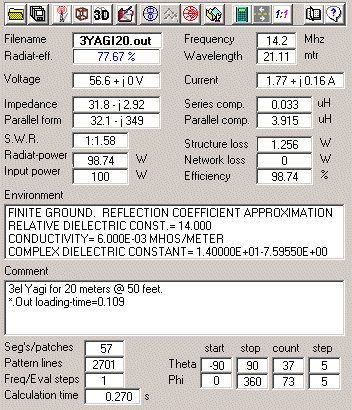
\includegraphics[width=.4\linewidth]{images/image002.png}
\caption{Ventana principal de 4NEC2.}
\end{figure}

\section{Características}

Algunas de las características que este software nos detalla en su
documentación (https://www.qsl.net/4nec2/) son:

\begin{itemize}
\item Las gráficas en 2D y 3D de visualización de estructuras geométricas.
\item Opción para arrastrar y soltar para poder modelar antenas.
\item Visualización interactiva de la Carta de Smith para barridos de
frecuencia.
\item Archivo de ayuda de manera contextual.
\end{itemize}

\section{Modelamiento de la antena}

Para el modelamiento de antenas debemos considerar distintos parámetros a tomar
en cuenta para diseñar una antena. Como se sabe hay fórmula sencillas que se
utilizan para hallar diseño de antenas (por ejemplo las dipolo) pero colocarlas
en un software como NEC2 facilita estos cálculos pues solo se pondrían ciertos
parámetros (como frecuencia y rango de radiación=) para que el mismo software
nos haga el análisis a partir del conocimiento previo que tenemos del programa.

NEC2 usa un análisis básico de la antena basado en el ``método de momentos'',
una técnica matemática donde subdivida una antena en pequeños segmentos para
calcular las propiedades mas apropiadas para cada caso. Los resultados pueden
ser sencillamente ajustados a las ecuaciones de ingeniería para resistencia del
material, carga del elemento y efectos de la tierra. 

\subsection{Modelamiento con Geometry Edit}

Con Geometry Editor se puede establecer la estructura geométrico de la antena.
Esta herramienta se encuentra dentro de al ventana Main en settings y se marca
Geometry Edit. Después de esto se presiona edit NEC and input file donde carga
un ejemplo.

Por ejemplo, si se quiere modelar un dipolo de $\lambda$.

\begin{figure}[H]
\centering
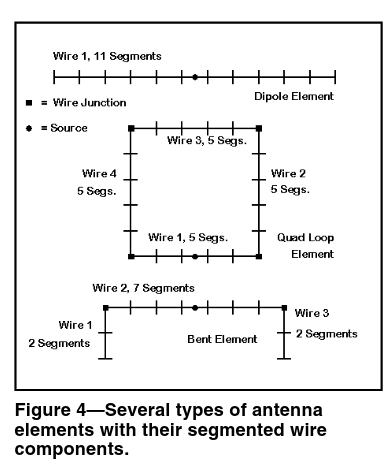
\includegraphics[width=.4\linewidth]{images/Captura de pantalla de 2021-09-12 23-21-26.png}
\end{figure}

En esta figura se pueden ver los distintos elementos, un dipolo, antenas
cúbicas de bucle y elementos doblados. Para formas que no son rectas en 4NEC2 se
debe poner un aproximado ya que es una figura no recta.

\section{Interfaz de usuario para 4nec2}

Al inicio el usuario tiene cuatro ventanas principales (y también accesos
rápidos a dichas ventanas. Las cuales son:

\begin{enumerate}
    \item Main (F2).
    \item Geometry (F3).
    \item Pattern (F4).
    \item Impedance (Imp/SWR/Gain) (F5).
\end{enumerate}

A continuación se puede ver una captura de pantalla de una maquina virtual con
4NEC2 instalado, donde se pueden apreciar las 4 ventanas ya abiertas.

\begin{figure}[H]
    \centering
    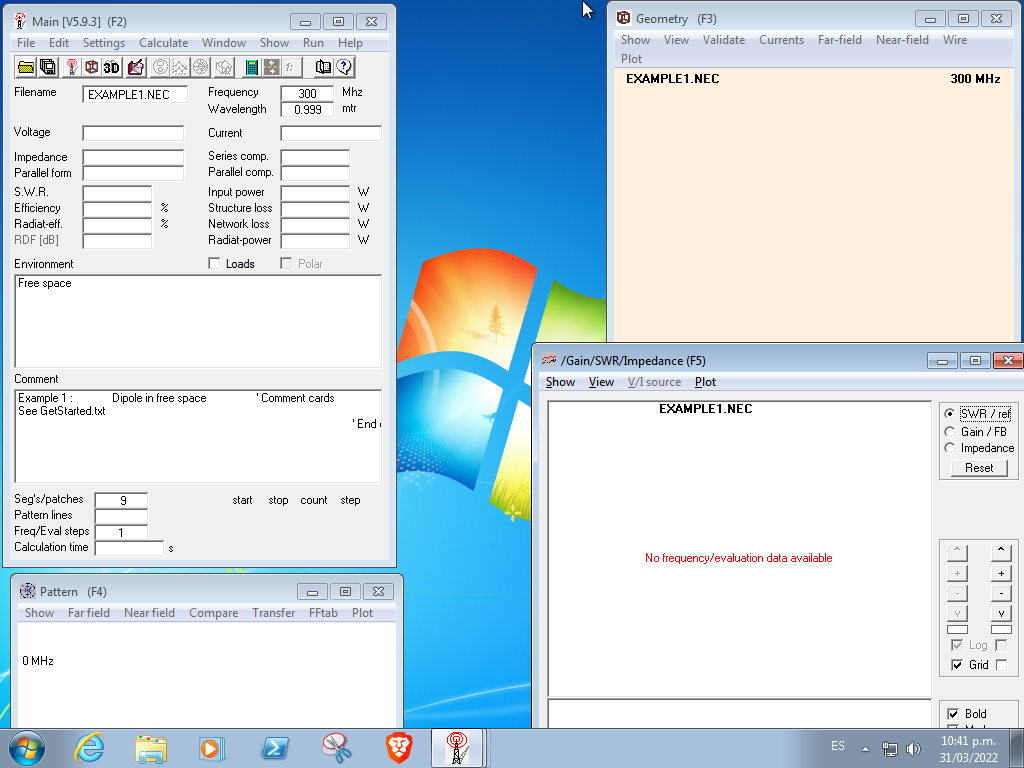
\includegraphics[width=.8\linewidth]{images/Screenshot_win7_2022-03-31_22_41_34.png}
    \caption{Captura de pantalla de las 4 ventanas ya ejecutadas.}
\end{figure}

\section{Como modelar antenas}

Lo importante antes de comenzar haciendo la modelación de las antenas es
conocer cual es nuestro entorno como por ejemplo saber que tipos de archivos
vamos a usar a editar, como lo veremos a continuación.

Hay muchas guías en internet pero en esta ocasión usaremos una guía disponible
en la página \href{https://leanpub.com/4nec2definitiveguide/read}{leanpub}.

\subsection{Archivos NEC}
Lo primero para poder hacer el modelamiento de la antena es reconocer como es
un archivo NEC (Numerical Electromagnetics Code ó Código Numérico
Electromagnético).

\begin{lstlisting}[language=,caption=Ejemplo de un archivo .NEC de una antena
logarítmica periódica.]
CM TESTEX5
CM 12 ELEMENT LOG PERIODIC ANTENNA IN FREE SPACE
CM 78 SEGMENTS. SIGMA=O/L RECEIVING AND TRANS. PATTERNS.
CM DIPOLE LENGTH TO DIAMETER RATIO=150.
CE TAU=0.93. SIGMA=0.70. BOOM IMPEDANCE=50. OHMS.
GW 1 5 0.0000 -1.0000 0.0000000 0.00000 1.0000 0.000 .00667
GW 2 5 -.7527 -1.0753 0. -.7527 1.0753 0. .00717
GW 3 5 -1.562 -1.1562 0. -1.562 1.1562 0. .00771
GW 4 5 -2.4323 -1.2432 0. -2.4323 1.2432 0. .00829
GW 5 5 -3.368 -1.3368 0. -3.368 1.3368 0. .00891
GW 6 7 -4.3742 -1.4374 0. -4.3742 1.4374 0. .00958
GW 7 7 -5.4562 -1.5456 0. -5.4562 1.5456 0. .0103
GW 8 7 -6.6195 -1.6619 0. -6.6195 1.6619 0. .01108
GW 9 7 -7.8705 -1.787 0. -7.8705 1.787 0. .01191
GW 10 7 -9.2156 -1.9215 0. -9.2156 1.9215 0. .01281
GW 11 9 -10.6619 -2.0662 0. -10.6619 2.0662 0. .01377
GW 12 9 -12.2171 -2.2217 0. -12.2171 2.2217 0. .01481
GE
FR 0 0 0 0 46.29 0.
TL 1 3 2 3 -50.
TL 2 3 3 3 -50.
TL 3 3 4 3 -50.
TL 4 3 5 3 -50.
TL 5 3 6 4 -50.
TL 6 4 7 4 -50.
TL 7 4 8 4 -50.
TL 8 4 9 4 -50.
TL 9 4 10 4 -50.
TL 10 4 11 5 -50.
TL 11 5 12 5 -50. ,0.,0.,0.,.02
EX 0 1 3 10 1 
RP 0 37 1 1110 90. 0. -5. 0.
EN
\end{lstlisting}

\section{Facilidades de procesado}

Se tiene dos formas para la simulación con NEC2, la primera es usando el editor
geométrico para desarrollar y modificar el modelado de una antena, es necesario
que se tenga por lo menos una variable a optimizar, estas variables pueden
estar en el bloc de notas o en el editor NEC2, el cual sería el modelado en
bloc de notas editor ``notepad''.

\section{Diseñando una antena}

Se pueden realizar dos tipos de diseño en el software, uno es mediante la
herramienta ``Geometry Edit'', en donde se puede establecer una estructura
geométrica y la otra es mediante la herramienta de ``Notepad ''.

\subsection{Modelado con Geometry Edit}

Con este tipo de modelado se establece la estructura geométrica de una antena.

Se tiene que editar  el archivo en formato NEC, como ya se ha visto
anteriormente, se presiona en el boton ``Edit NEC and input file''.

Usando como ejemplo una antena dipolo $\lambda$

\end{document}
